\section{UD and SUD model comparison}
The first hypothesis this work aims to verify is that the parsing model trained to annotate according to the SUD scheme will perform better than the one annotating according to the UD scheme. 

Corpora chosen for training are all split into three parts each: training, validation and testing. The training and validation splits were used during the training process. For evaluation, the models predicted the correct annotation for every sentence in the testing split. Those predictions were then compared to the original annotations for those sentences and two metrics were calculated: unlabelled and labelled attachment score. Unlabelled attachment score, or UAS, is the percentage of words in a sentence that have a correctly predicted governor. Labelled attachment score, or LAS, is the percentage of words that have a correctly predicted governor as well as the dependency label that connects that word to its governor. Those scores for both the UD and SUD model are presented in Table \ref{tab:mcnemar} along with the differences between those accuracies. Both of the differences are significant and in both cases it is in favour of the UD model.\footnote{Evaluation was performed using the \texttt{conll18\_ud\_eval.py} script from the study conducted by \cite{tuo:prz:lac:21}, found in the related repository: \url{https://github.com/ryszardtuora/ud_vs_sud}.}

\begin{table}[h!]
\centering
\begin{tabular}{|| c c c | c c c ||}
\hline
& UAS & & & LAS & \\
\hline
UD & SUD & $\Delta$ & UD & SUD & $\Delta$ \\
\hline \hline
89.75 & 88.95 & \textbf{0.8} & 87.29 & 86.80 & \textbf{0.49} \\
\hline
\end{tabular}
\caption{\centering Attachment scores for the models trained on combined UD and SUD corpora and the difference between them}\label{tab:mcnemar}
\end{table}

Thus the first hypothesis was not confirmed, but the differences between the models trained on UD and SUD were small enought to continue the study. 

\section{Governor's impact on the coordination}
\begin{figure}[hbt!]
    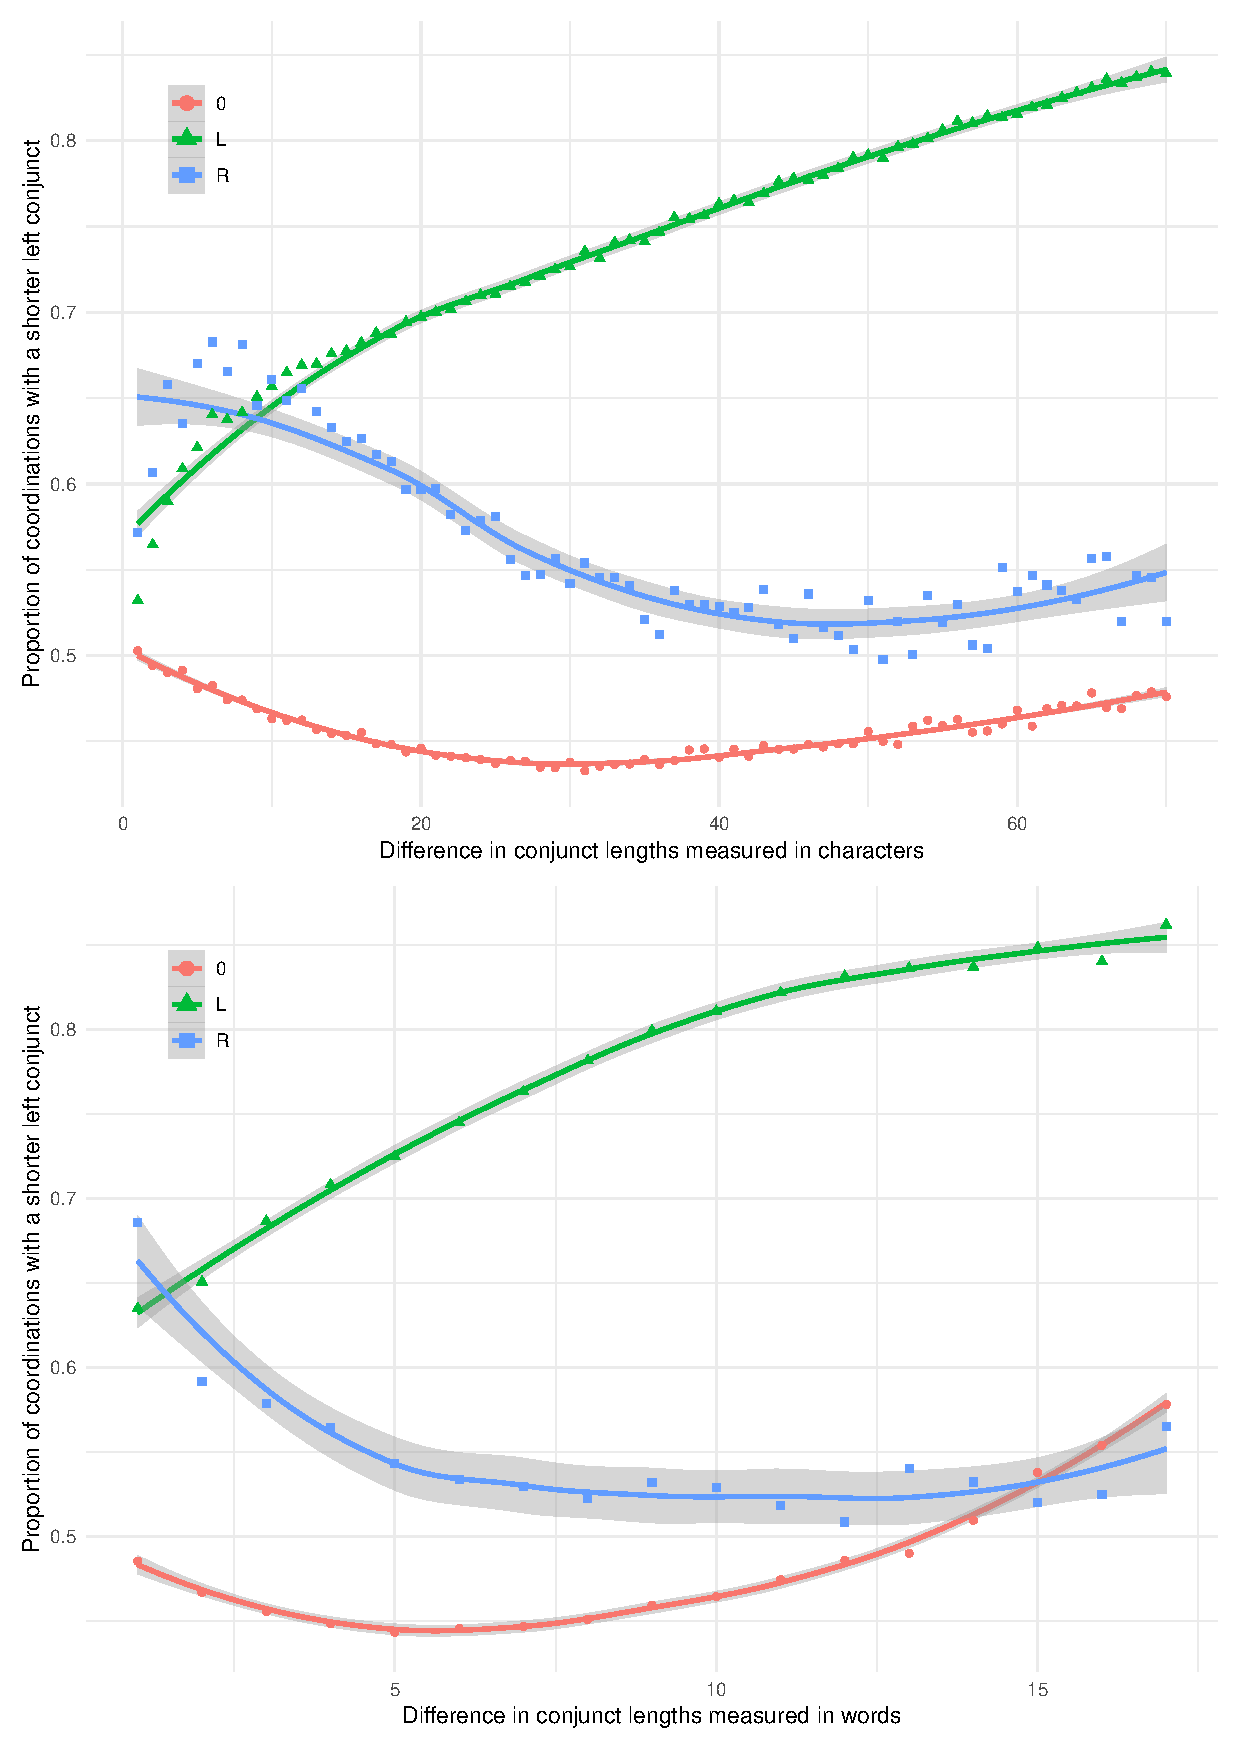
\includegraphics[width=\textwidth]{inputs/observed.pdf}
    \caption{\centering Observed and loess-smoothed proportions of coordinations with shorter left conjuncts depending on the length difference between the conjuncts and on the position of the governor}\label{fig:observed}
\end{figure}

The second hypothesis tested here is that placement of the shorter conjunct in a coordination is affected by the governor position and the length difference between the conjuncts. Figure \ref{fig:observed} shows the observed proportions of coordinations with shorter left conjuncts depending on the length difference between the conjuncts, grouped by the possible positions of the governor. Regardless of the measure, the proportion of coordinations with shorter left conjuncts increases steadily when the governor is on the left. When there is no governor the proportion decrases at first and starts to grow around length differences equal to 30 characters or 7 words. Similarly with the governor on the right, the proportions decrease initially and rise slightly with bigger length differences, but the changes happen at different rates between the two presentes measures.

Figure \ref{fig:logit} shows the results of fitting logistic regression models to the observations presented in Figure \ref{fig:observed}. Here the slopes are more consistent between the utilised measures. When the governor is on the left, the slopes are positive, when there is no governor they are slightly negative and when the governor is on the right they are also negative, but this time much steeper. 

\begin{figure}[hbt!]
    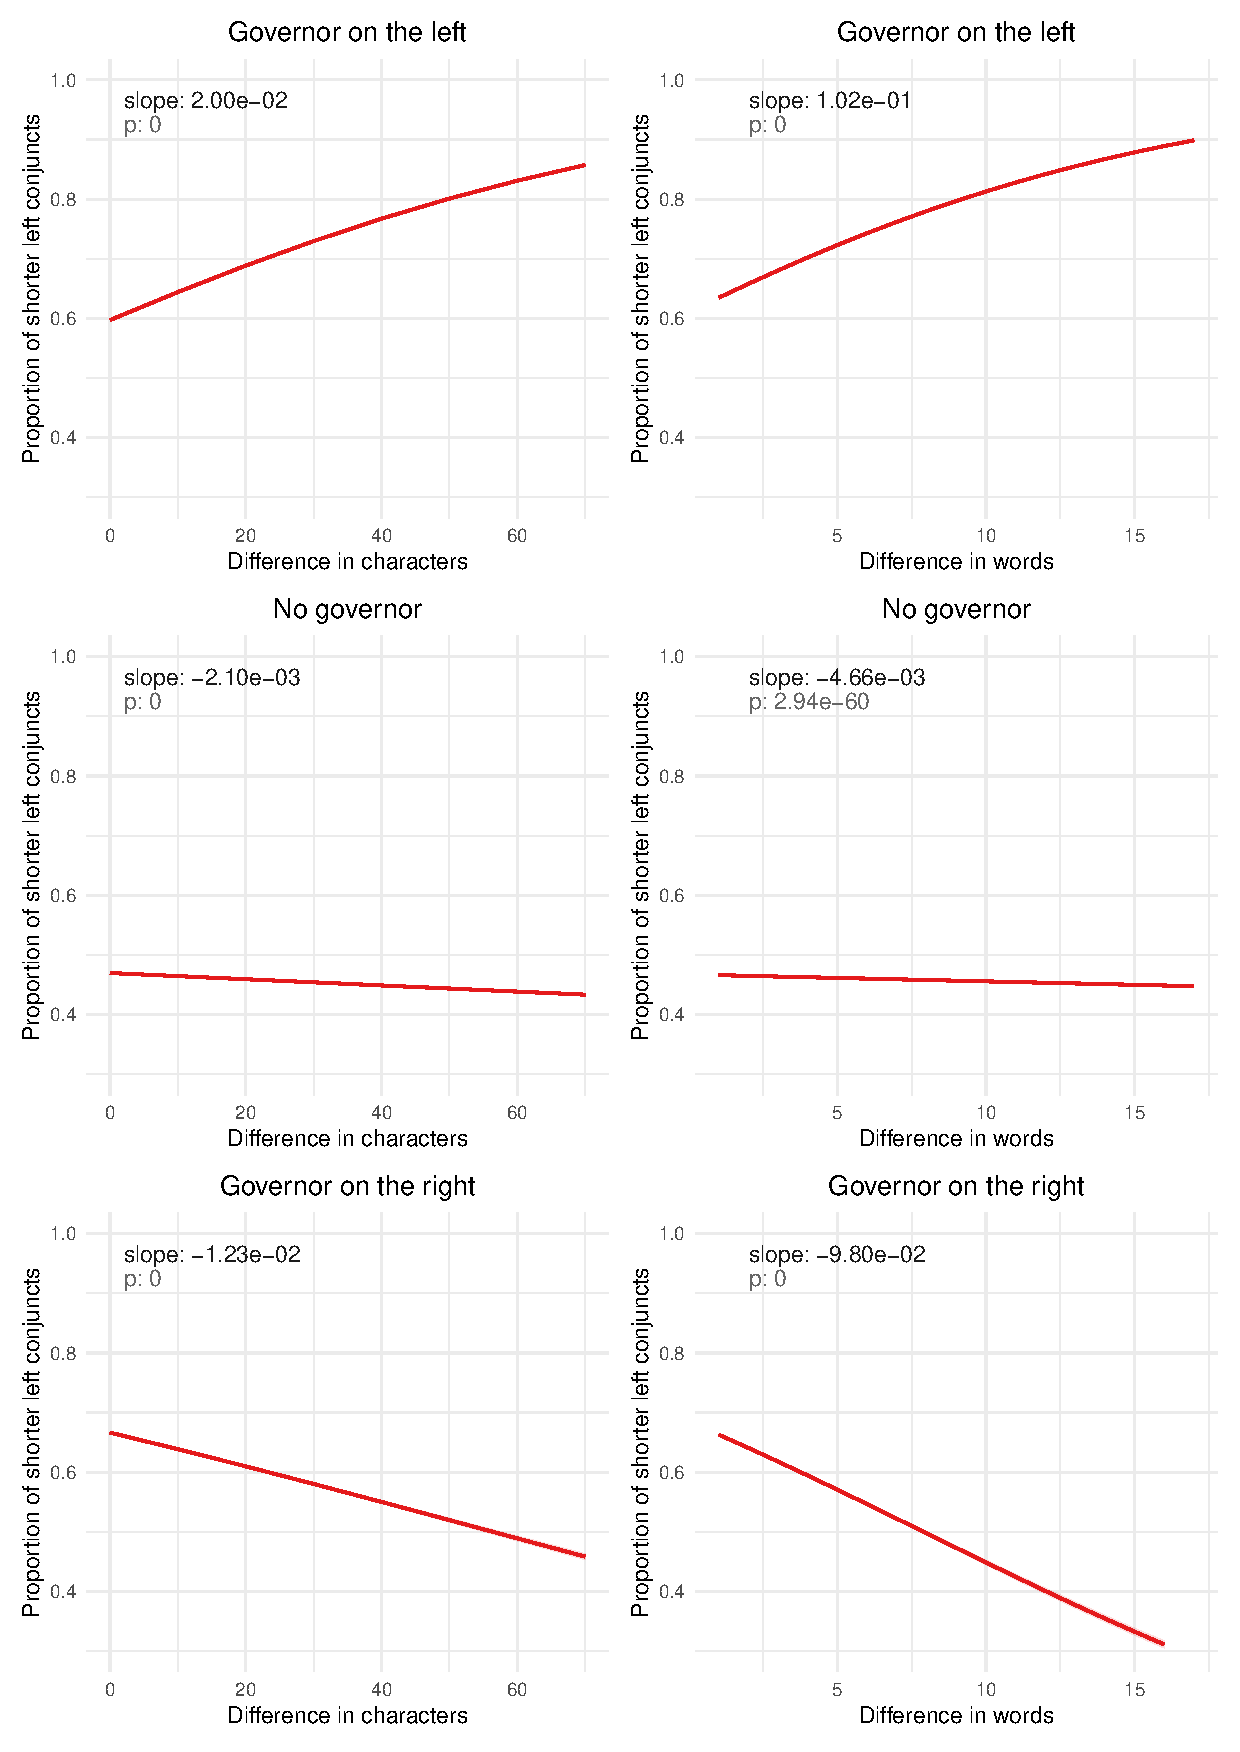
\includegraphics[width=\textwidth]{inputs/modelled.pdf}
    \caption{\centering Modelled proportions of coordinations with shorter left conjunct depending on the length difference between the conjuncts}\label{fig:logit}
\end{figure}

The Hosmer-Lemeshow test \citep{hoslem} was used to test the goodness of fit of the models presented in Figure \ref{fig:logit}.
The null hypothesis of the test is that the observed and predicted proportions are the same. The test was performed using R's \texttt{ResourceSelection::hoslem.test}. In the models fitted to data gathered here, the proportion of coordinations with shorter left conjuncts is predicted based on the length difference between the two conjuncts. Those proportions are arranged in an ascending order and grouped into 10 percentile groups. Then the Hosmer-Lemeshow statistic is calculated using the formula in (\ref{eq:hoslem}). 

\begin{equation}\label{eq:hoslem}
H = \sum_{g=1}^{G}\left(\frac{(O_{1g}-E_{1g})^2}{E_{1g}} + \frac{(O_{0g}-E_{0g})^2}{E_{0g}}\right)
\end{equation}

The results of the tests run on all of the models are presented in (\ref{tab:hoslem}).

\begin{table}[hbt!]
\begin{tabular}{l|r|r|r|}
model & X-squared & degrees of freedom & p-value\\\hline
L-char & 9762.6 & 8 & $<$ 2.2e-16\\
R-char & 2781.5 & 8 & $<$ 2.2e-16\\
0-char & 4926.6 & 8 & $<$ 2.2e-16\\
L-words & 460.9 & 4 & $<$ 2.2e-16\\
R-words & 3490.8 & 2 & $<$ 2.2e-16\\
0-words & 4142.6 & 5 & $<$ 2.2e-16
\end{tabular}
\caption{Results of the Hosmer-Lemeshow test conducted on the logistic regression models.}
\label{tab:hoslem}
\end{table}

\begin{figure}
    \hspace{-.1\textwidth}
    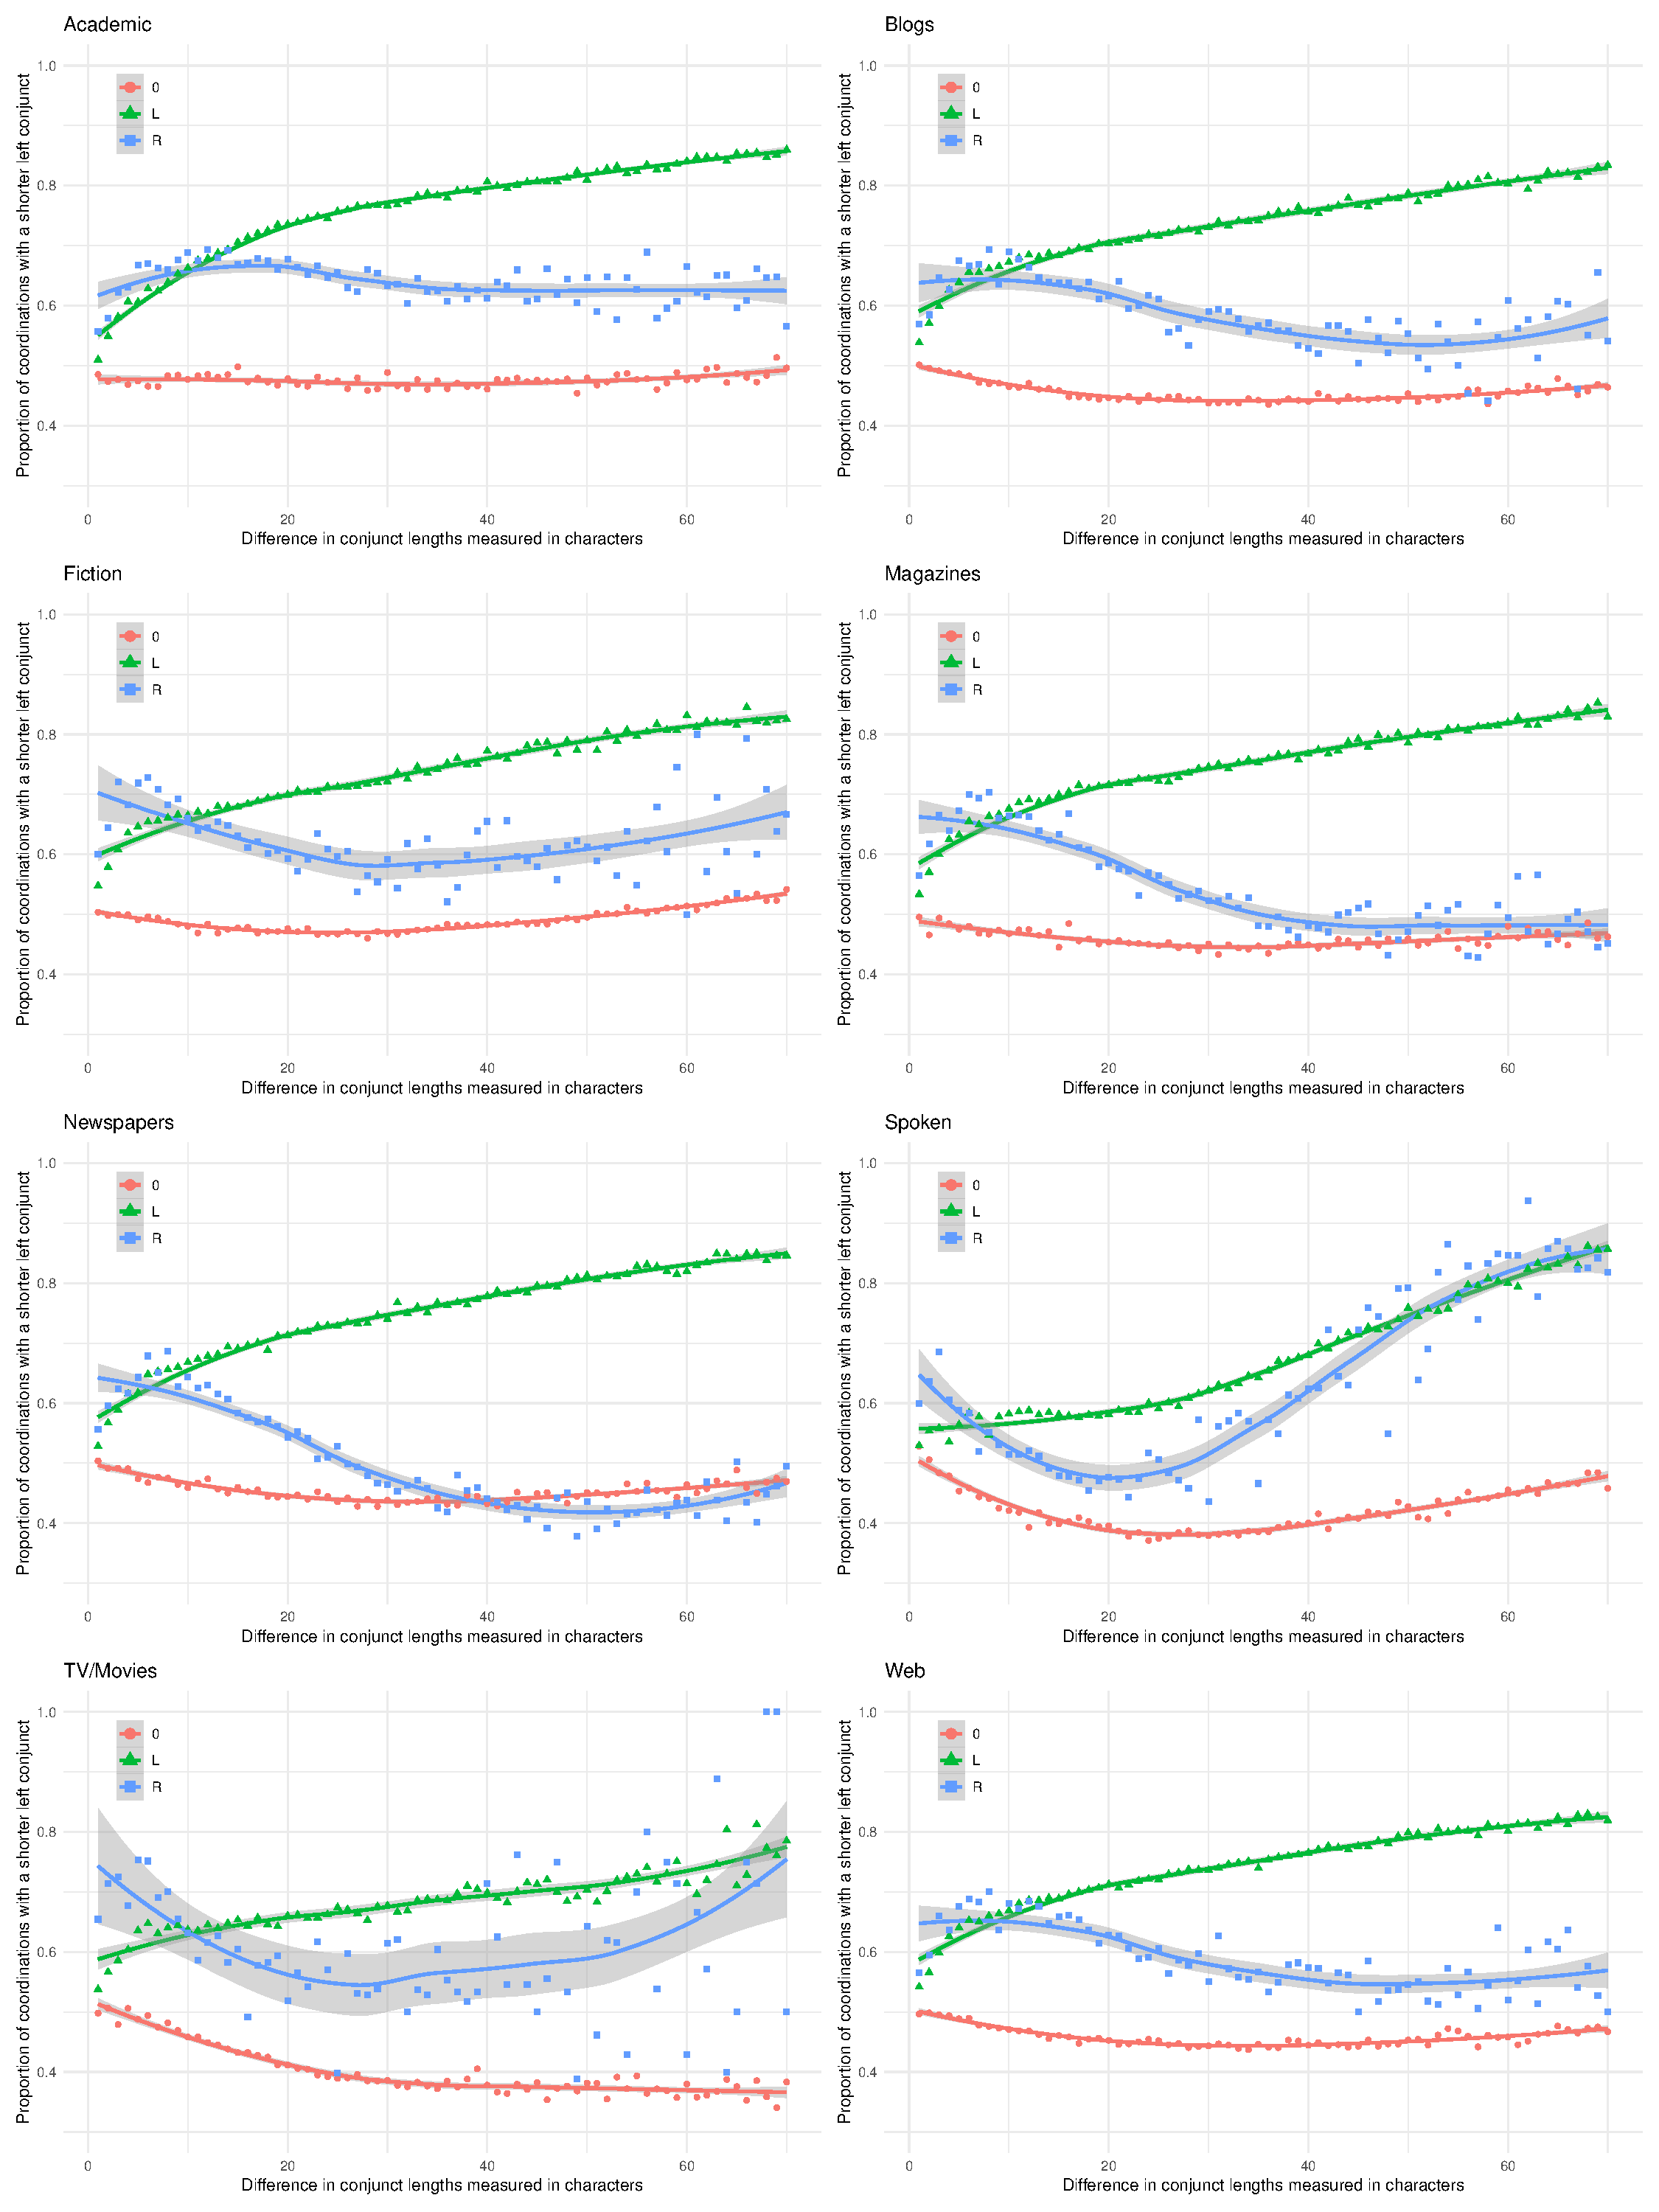
\includegraphics[width=1.2\textwidth]{inputs/genres.pdf}
    \caption{\centering Observed and loess-smoothed proportions of coordinations with shorter left conjuncts depending on the length difference between the conjuncts and on the position of the governor in different genres}
\end{figure}
